\documentclass[10pt]{article}
\usepackage{graphicx}
\usepackage{amssymb}
\usepackage[fleqn]{amsmath}
\usepackage{nccmath}
\usepackage{cases}
\usepackage{hyperref}
\usepackage{multicol}
\usepackage{tikz}
\usepackage{pgfplots}
\usepackage{enumitem}
\pgfplotsset{compat=1.18}
\usepackage{float}
\usepackage{pdfpages}
\DeclareMathOperator*{\lcm}{lcm}

\title{\bf Math 116: Problem Set 6}
\date{2/27/2024}
\author{\bf Owen Jones}
\begin{document}
\maketitle
\begin{enumerate}[label= \arabic*.]
    \item \begin{enumerate}
        \item If $\gcd(e,24)=1$, then $\gcd(e,3)=1$ and $e$ is odd. \\
        By Fermat's Little Theorem, $e^2\equiv 1\pmod{3}$\\
        $\begin{cases}
            e^2\equiv 16m^2+24m+9\equiv 1\pmod{8} & \text{ if }e\equiv 3\pmod{4}\\
            e^2\equiv 16m^2+8m+1\equiv 1\pmod{8} & \text{ if }e\equiv 1\pmod{4}
        \end{cases}$\\
        Because $e^2=1\pmod{24}$ satisfies the system of conguences
        \begin{align*}
            &e^2\equiv 1\pmod{3}\\
            &e^2\equiv 1\pmod{8}
        \end{align*} the CRT states $e^2\equiv 1\pmod{24}$ must be the unique solution to the system.
        \item $\phi(35)=\phi(5)\cdot\phi(7)=24$. 
        Thus, $ed\equiv 1\pmod{24}$.
        However, we know from part (a) that if $e$ and $24$ are coprime, $e^2\equiv 1\pmod{24}$.\\ 
        Thus, $c^e\equiv {(m^e)}^e\equiv m^{e^2}\equiv m^{\phi(35)k}\cdot m\equiv m\pmod{35}$
    \end{enumerate}
    \item $\gcd(e,(p-1)(q-1)(r-1))=1$ and $\gcd(d,(p-1)(q-1)(r-1))=1$.
    \item No. It is equivalent to using a single encryption exponent $e^*=e_1\cdot e_2$. 
    It is not any more difficult to find a $d$ s.t $de^*\equiv 1\pmod{\phi(n)}$ i.e it still only depends on how difficult it is to factor $n$.
    \item From the information given $n\mid (516107\cdot 187722-14)(516107\cdot 187722+14)$. It follows $\gcd(n,516107\cdot 187722-14)=1129$ which is a non-trivial factor of $n$, the other being $569$.\\
    \begin{align*}
        &(516107\cdot 187722-14)=642401\cdot 150816+289024\\
        &642401=2\cdot 289024+64353\\
        &289024=4\cdot 64353+31612\\
        &64353=2\cdot31612=1129\\
        &31612=28\cdot 1129
    \end{align*}
    \item $m_B-m_A\equiv p\cdot p^{-1}\pmod{n}$ by the CRT where $p\cdot p^{-1}\equiv 1\pmod{q}$. 
    $0<p\cdot p^{-1}<n$ because $0<p^{-1}<q$. 
    It follows $\gcd(p\cdot p^{-1},n)=p$ gives one of the non-trivial factors of $n$.
    \item \begin{enumerate}
        \item If $\alpha$ is a primitive root, then $\alpha^{L_\alpha(\beta_1\cdot\beta_2)}\equiv\alpha^{L_\alpha(\beta_1)+L_\alpha(\beta_2)}\pmod{p}$ iff $L_\alpha(\beta_1\cdot\beta_2)\equiv L_\alpha(\beta_1)+L_\alpha(\beta_2)\pmod{p-1}$.
        Because $\alpha$ is a primitive root, $L_\alpha$ is onto.
        $\alpha^{L_\alpha(\beta_1\cdot\beta_2)}\equiv\beta_1\cdot \beta_2\equiv \alpha^{L_\alpha(\beta_1)}\cdot\alpha^{L_\alpha(\beta_2)}\equiv \alpha^{L_\alpha(\beta_1)+L_\alpha(\beta_2)}\pmod{p}$.
        \item Since $\alpha$ is not necesarily a primitive root, $k\le p-1$ where $k$ is the smallest integer s.t $\alpha^k\equiv 1\pmod{p}$.
        Let $x=L_\alpha(\beta_1\cdot\beta_2),y=L_\alpha(\beta_1)$, and $z=L_\alpha(\beta_2)$ for $0\le x,y,z<k$. 
        It follows $\alpha^x\equiv \beta_1\cdot\beta_2\equiv \alpha^y\cdot\alpha^z\pmod{p}$.
        Because $a^{x-y-z}\equiv1\equiv \alpha^k\pmod{p}\Rightarrow x\equiv y+z\pmod{k}$. 
        Thus, $L_\alpha(\beta_1\cdot\beta_2)\equiv L_\alpha(\beta_1)+L_\alpha(\beta_2)\pmod{k}$.
    \end{enumerate}
    \item \begin{enumerate}
        \item $L_2(24)\equiv 3L_2(2)+L_2(3)\pmod{100}$. 
        $L_2(2)=1\Leftrightarrow 2^1\equiv 2\pmod{101}$ trivially. 
        Thus, $L_2(24)\equiv 72\pmod{100}$.
        \item Given $5^3\equiv 24\pmod{101}$, 
        it follows $2^{L_2(24)}\equiv 2^{3L_2(5)}\pmod{101}$. 
        Thus, $L_2(24)\equiv 3L_2(5)\equiv 3\cdot 24\equiv 72\pmod{100}$.
    \end{enumerate}
    \item Given $3^6\equiv 44\pmod{137}$ and $3^{10}\equiv 2\pmod{137}$, it follows $L_3(44)=6$ and $L_3(2)=10$ $L_3(44)-2L_3(2)\equiv L_3(11)\equiv -14\pmod{136}$. 
    Thus, $L_3(11)\equiv 122\pmod{136}$.
    \item \begin{enumerate}
        \item Discrete logarithms are an example of a one way function. Computing $b^y\pmod{p}$ to check password against the list of encrypted passwords is computationally easy. 
        However, given the list of encrypted passwords, it is computationally difficult to deduce the password, $x$, from $b^x\pmod{p}$ because checking every $x$ between $0$ and $p-1$ would take centuries to compute when $p$ is of the order of magnitude $10^{499}$.
        \item The system in part (a) would not be secure if $p$ was a $5$ digit number because an exhaustive search of every $x$ between $0$ and $p-1$ is feasible with a sufficiently fast computer. Thus, this system would be weak to a brute force attack.
    \end{enumerate}
    \item If $r=7\Rightarrow r^{-1}\equiv 5\pmod{17}$.\\
    Thus, ${(r^{-1})}^a\beta^k m\equiv m\equiv 5^6\cdot 6\equiv 12\pmod{17}$.\\
    Hence, $m=12$.
    \item \begin{enumerate}
        \item If $0\le m<n_i$ for $i=1,2,3$, 
        $0\le m^2<mn_1<n_1n_2\\
        \Rightarrow 0\le m^3<m^2n_3<n_1n_2n_3$.\\
        Thus, $0\le m^3<n_1n_2n_3$.
        \item Let $N=n_1n_2n_3$,
        $z_i=\frac{N}{n_i}$,
        $y_i\equiv z_i^{-1}\pmod{n_i}$\\
        Thus, $c_1y_1z_1+c_2y_2z_2+c_3y_3z_3$ satisfies the system of conguences.\\
        Let $m^3\equiv c_1y_1z_1+c_2y_2z_2+c_3y_3z_3\pmod{n_1n_2n_3}$ be the smallest positive integer that satisfies the congruence relation.
        \item $m=230520182119202018051420$ WETRUSTTRENT\\ Found using bisection method.
    \end{enumerate}
    \item \begin{enumerate}
        \item $p=3994211774931437561721507289\\ q=771813803019901406912522267$
        \item $m=805250221040425$ HEYBUDDY
    \end{enumerate}
    \item $3^{1234}\equiv 8576\pmod{53047}$
    \item\begin{enumerate}
        \item $2^{2000}\equiv 3925\pmod{3989},2^{3000}\equiv1046\pmod{3989}$
        \item $L_2(3925\cdot 1046)\equiv L_2(3925)+L_2(1046)\equiv 5000\equiv1012\pmod{3988}$.
        Thus, $L_2(3925\cdot 1046)=1012$.
    \end{enumerate}
\end{enumerate}
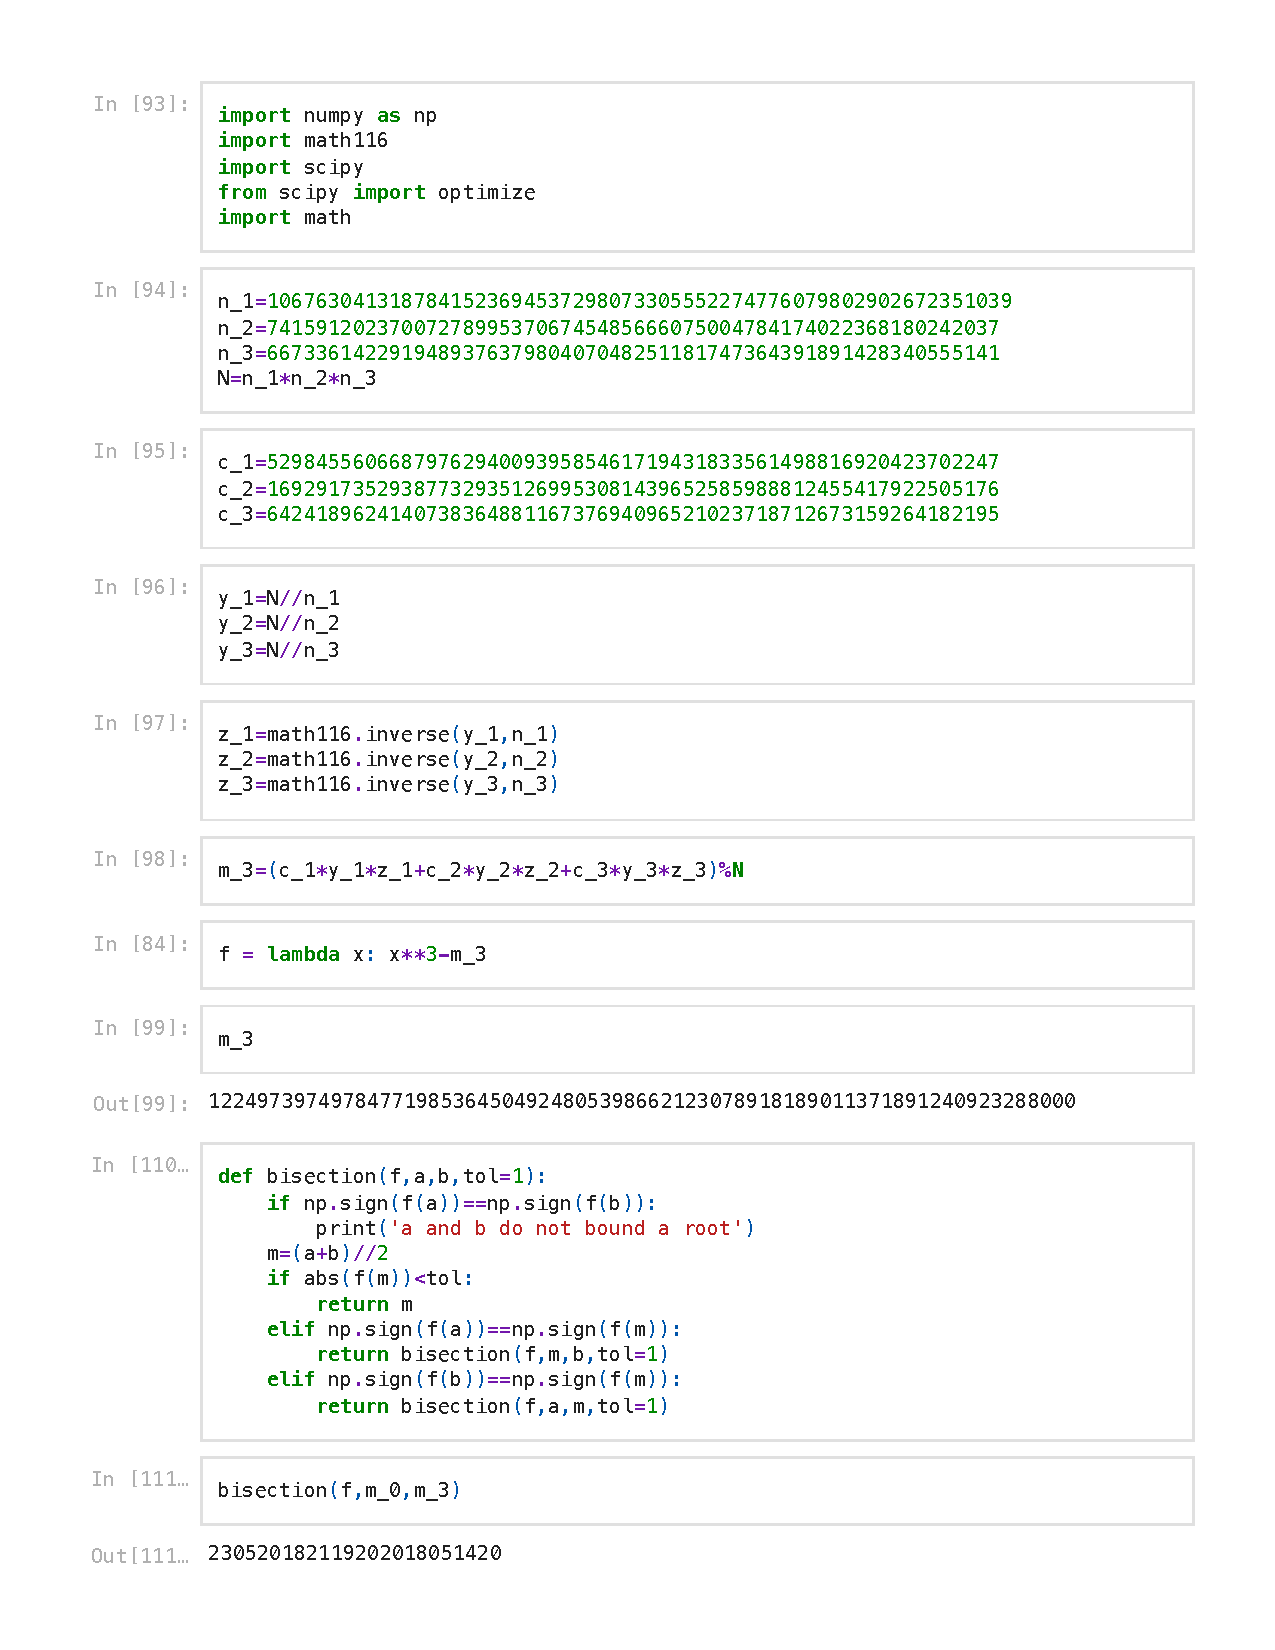
\includepdf[pages=-]{Math_116_homework_6_python.pdf}
\end{document}